% \section{multi-tier Fog computing model}
% \label{sec:fog-model}

\subsection*{Research Goals}
\label{sec:research-goals}

This project aims to design a reliable and high-quality DASH-based video delivery to be used in Smart City Environments~\cite{gamaUCC2019, KreuzbergerWorkshop2016}. The proposed scheme will take advantage of several network-related technologies such as Cloud, Fog, and Edge Computing, as well as intelligent service placement and chaining. Figure~\ref{fig:scenario-arch} depicts, on its left-hand side, a multi-tier network architecture, which is composed of a heterogeneous set of devices and applications using distributed computing resources through a multi-access communication technology, such as 5G and WiFi. This project proposes to extend DASH video streaming to support simultaneous multipath connectivity~\cite{poliakovPHD2018, Velasquez2018}.

The right-hand side of Figure~\ref{fig:scenario-arch} describes part of the parameters that should be assessed to define which video services are needed to be deployed along with the most suitable tier to deploy each of them. Note that the parameters in the bottommost tier for feedback differ from those of other tiers. Initially, the assessed parameters considered include the user's profile, the load of the local cell, the link quality, the motion complexity of the videos, and also smart city details such as the location and the traced route in case of users with mobility. Some of the nodes can be stationary, but others can range from low to high mobility patterns, which can be taken into account to improve quality of video delivery.

\vspace{0.8cm}
\begin{figure*}[htpb]
	\centering
	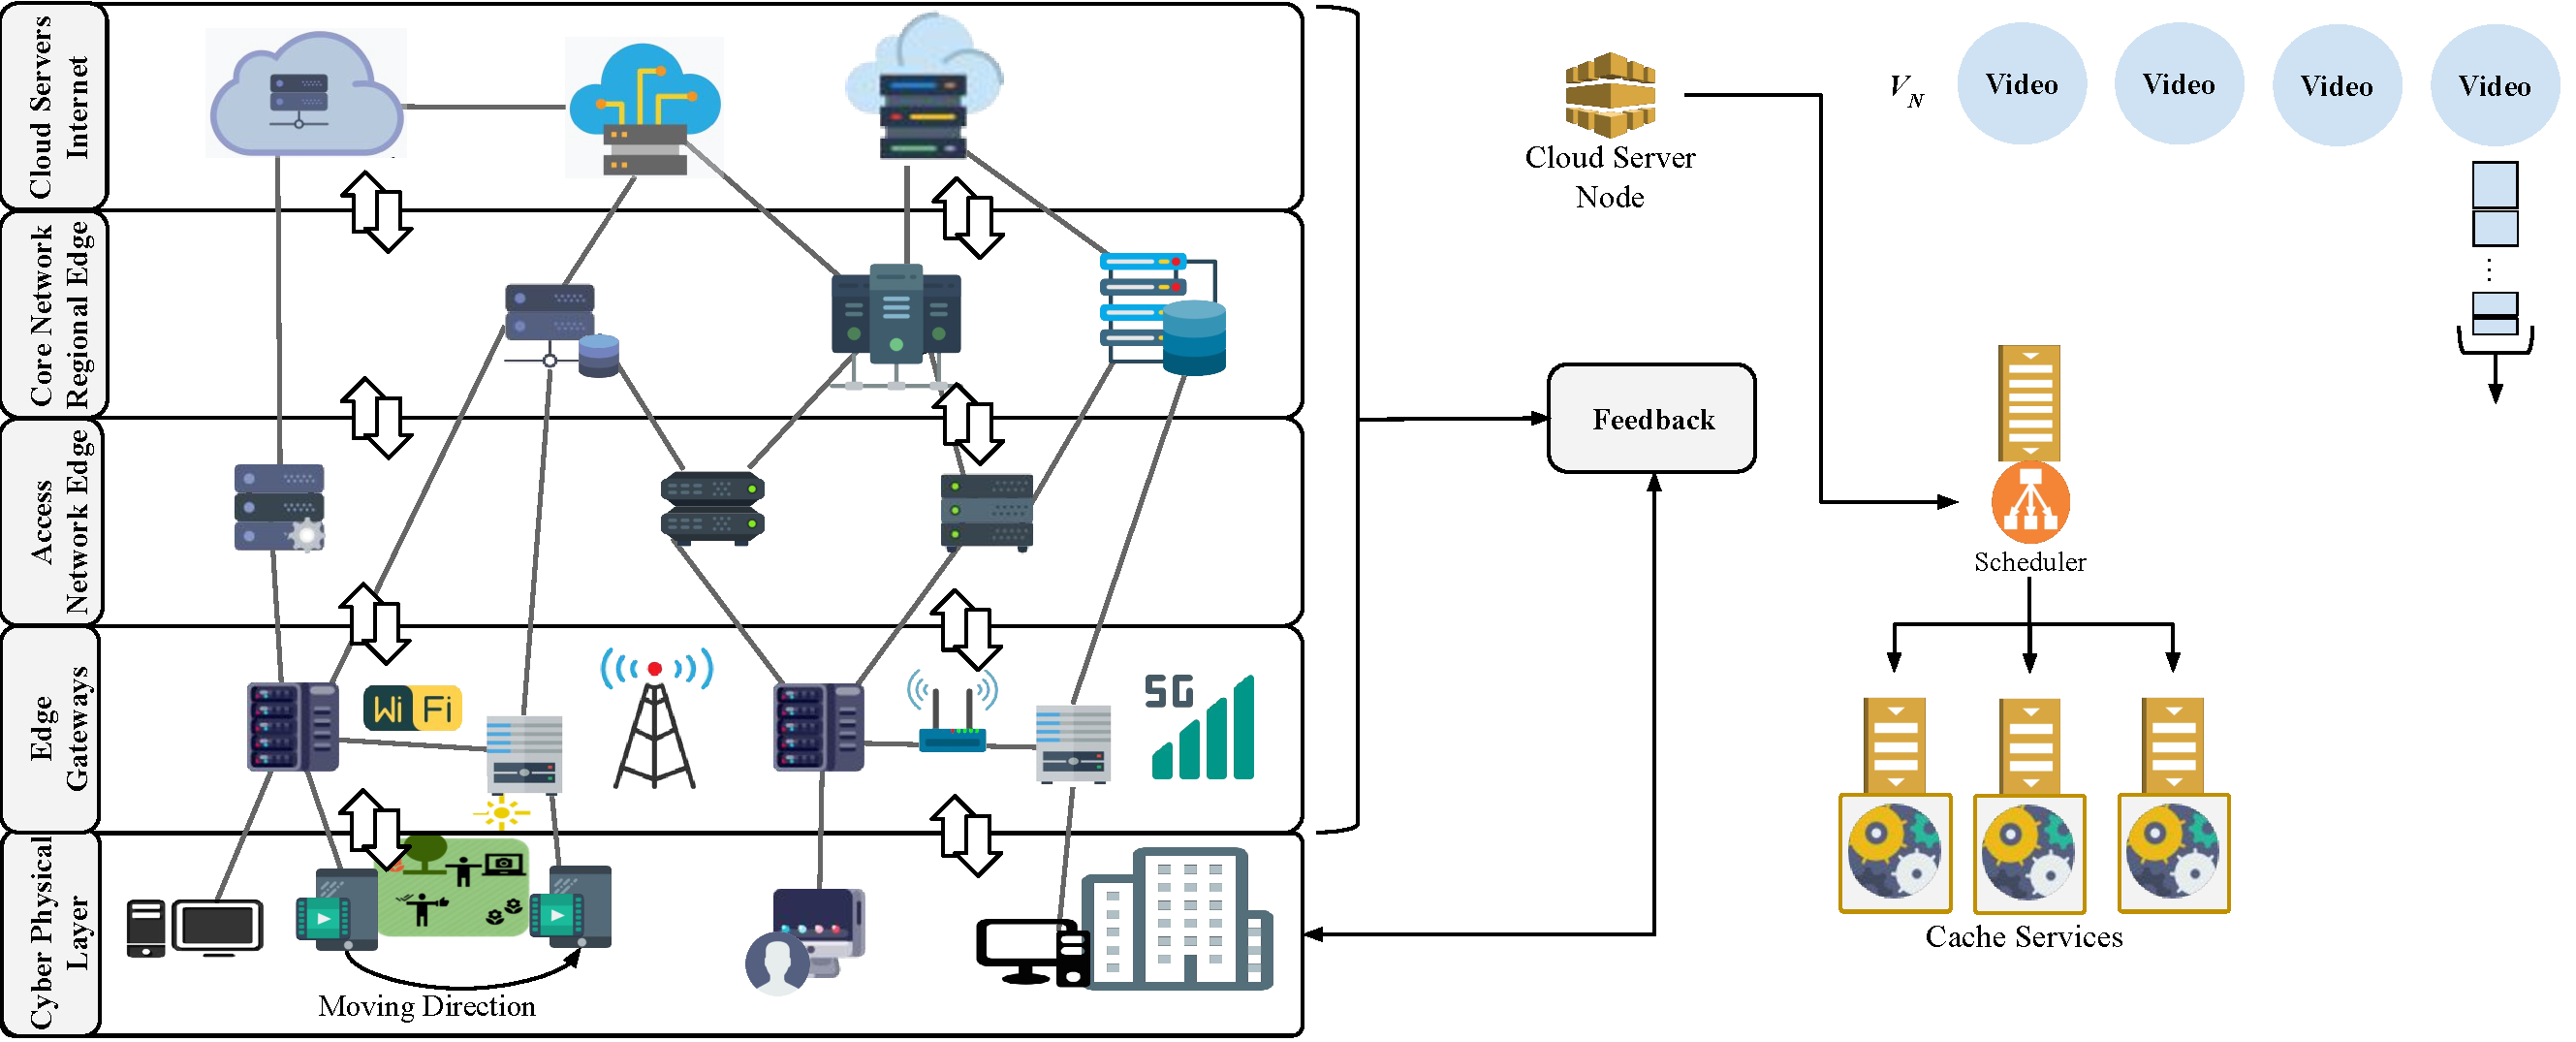
\includegraphics[width=1.0\textwidth]{images/scenario_incomplete}
% 	\vspace{-1cm}
	\caption{DASH-based Adaptive Multimedia Delivery System in an Smart City Environment.}
	\label{fig:scenario-arch}
\end{figure*}

Given the aforementioned multi-tier edge/cloud environment and service model architecture, this work aims to tackle some of the following research questions:~\textit{i)} How to determine the best tiers for video services placement?~\textit{ii)} How unsolicited video chunks should be distributed in the edge/cloud hierarchy considering user location information and estimates on future user location in real time? ~\textit{iii)} How to facilitate video streaming through multiple sources concurrently?~\textit{iv)} How bitrate adaptation algorithms can be impacted by video chunk size in a multi-tiered architecture?
